%*****************************************
\chapter{Hypothesis Testing: Parametric Tests}\label{hyp:parametric}
%*****************************************
\section{Introduction}

An important function for statistical analysis is to test a hypothesis to see if it adequately explains some observed phenomenon. The statistical processes for quantitative data are introduced in this lab and the processes for qualitative data are in \nameref{hyp:nonparametric} on \pageref{hyp:nonparametric}.\footnote{The definitions of ``hypothesis'' and the various data types are found in the \nameref{int:introduction}, beginning on page \pageref{intro:Hypothesis}.} 

\section{ANOVA}

\textit{More Than 2 Groups : Ratio/Interval Data}

An Analysis of Variance (ANOVA) is used to analyze the difference in three or more groups of observations. For example, imagine three groups of students were in the same class and one group was required to attend tutoring once a week, a second group twice a week, and a third group never. The null hypothesis ($ H_{0} $) is ``The amount of tutoring does not significantly change a student's score on the final exam.'' The alternate hypothesis ($ H_{a} $) is ``More frequent tutoring significantly changes a student's score on the final test.'' After the final exam was graded, an ANOVA could be administered and if that showed the test scores for those three groups of students had a significant difference then the null hypothesis would be rejected in favor of the alternate hypothesis.

\section{t-test - Independent} 

\textit{2 Groups : Ratio/Interval Data : Not Paired}

An independent t-test is one of the most commonly used measures of the difference between two groups. One example of an independent t-test is to compare the spending habits of two similar groups of people. For example, do the residents of Tucson spend more on dining out than the residents of Phoenix? The null hypothesis ($ H_{0} $) is ``People in Phoenix and Tucson spend the same amount of money when dining out.'' The alternate hypothesis ($ H_{a} $) is ``People in Phoenix and Tucson spend different amounts of money when dining out.'' Imagine that the dining bills of $ 100 $ people from both cities were recorded and it was discovered that the mean bill in Phoenix is \$$ 15.13 $ and in Tucson is \$$ 12.47 $. A t-test would determine if there a significant difference in those two numbers, thus rejecting the null hypothesis, or if this is just a statistical fluke.

\section{t-test - Paired}

\textit{2 Groups : Ratio/Interval Data : Paired}

A paired t-test is commonly used to compare the difference between two groups that are paired in some way. Typically, this is used in a test-retest type of experiment. Imagine that a group of students were given a pretest, taught a lesson, and then given a post-test. A paired t-test would be used to compare each student's pretest and post-test scores to see if there is a significant difference in the means for the two tests. Probably the most common use of a paired t-test is in medical drug trials. Typically, some physiological measurement is made of a group of patients (a blood pressure, for example), then the group is split in half and one group receives the drug being tested while the other receives a placebo. At the end of the trial the same measurement is made that was used during the pre-treatment and a paired t-test is used to compare the results of each individual in the two groups to see if the drug brought about a significant improvement.

\section{Procedure}

\texttt{SOFA} makes it easy to complete any of the statistical tests listed in this lab exercise. A Wizard provides help in selecting an appropriate test but users can also manually select and configure whatever test they need.

\subsection{ANOVA}

\begin{enumerate}
  \item Start \texttt{SOFA} and click the "Statistics" button
  \item Select "ANOVA" from the Statistical Test list at the top of the window and then click the "Configure Test" button
  \item Data Source Table: email
  \item Averaged variable: Line\_Breaks
  \item Algorithm: Speed 
  \item Group By variable: Spam
  \item From Group: No
  \item To: Yes
  \item Click ``Show Results''
  
  \begin{figure}[H]
    \begin{center}
      \fbox{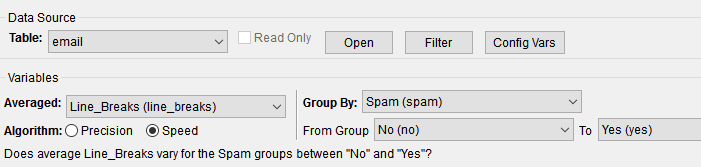
\includegraphics[width=\linewidth]{gfx/hyppara010}}
      \caption{Setting Up the ANOVA Test}
    \end{center}
  \end{figure}
  
  \item The ANOVA test generates a lot of information.
  
  \begin{enumerate}
    \item \textbf{ANOVA Table}. This displays information about two broad partitions of the calculated data. The ``Between'' Source are values calculated when comparing two (or more) groups and the ``Within'' Source are values calculated within a single group. 

    \begin{figure}[H]
      \begin{center}
        \fbox{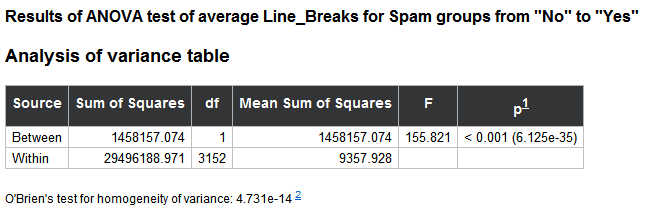
\includegraphics[width=\linewidth]{gfx/hyppara015}}
        \caption{ANOVA Table}
      \end{center}
    \end{figure}
  
      \begin{itemize}
        \item \textbf{Sum of Squares}. Each value in both groups is subtracted from the mean of that group, then that number is squared (to eliminate negative values), and, finally, all of the squared are summed. For the purposes of this exercise the Sum of Squares is of little value.
        \item \textbf{df}. The degrees of freedom is calculated for the groups being analyzed. The degrees of freedom is one less than the number of groups.\footnote{The concept of Degrees of Freedom is explained in Lab \ref{cor:degrees_of_freedom}, page \pageref{cor:degrees_of_freedom}.}
        \item \textbf{Mean Sum of Squares}. This is the mean of the sum of the squares. This is calculated as the sum of squares divided by the degrees of freedom. (Note: the Mean Sum of Squares for the Within Source is frequently referred to as the ``residuals'').
        \item \textbf{F}. This is the value of the ``F-Test'' for this ANOVA. An F-Test is the ratio between two mean square values and used to indicate if the variance between groups is significantly different from the variance within the groups. In general, if the null hypothesis is true then the F-Test value will be close to one, that is, there is not much difference in the variance between groups when compared to the variance within a group. In the example calculated for this exercise, the F-Test value is $ 155.821 $ which is much larger than one and would indicate that there is a significant difference in the variance of the ``no'' and ``yes'' groups.
        \item \textbf{p value}. This is computed from the F-value and is used to determine if the null hypothesis can be rejected.\footnote{The concept of P-Value was explained in Lab \ref{cor:chi_square}, page \pageref{cor:chi_square}.} \textit{Most research reports include only the P-Value rather than all of the other calculated statistics since it summarizes the result into a single easy-to-understand number.} In most cases a P-Value less than $ 0.05 $ ($ 5\% $) indicates that there is a significant difference in the groups being compared. In the example calculated for this exercise, the P-Value is far less than $ 0.05 $ (at $ 6.125 \times 10^{-35} $) so the result is significant and the null hypothesis can be rejected.
        \item \textbf{O'Brien's Test}. This test is commonly used to indicate if the variances within two groups is significantly different. If the value of O'Brien's test is less than $ 0.05 $ ($ 5\% $) then the difference in the two variances is significant. In the example calculated for this exercise, O'Brien's test is well under $ 0.05 $ (at $ 4.731 \times 10^{-14} $), so the difference in the variance within the ``no'' group and ``yes'' group is significant.
      \end{itemize}
    
    \item \textbf{Group Summary Details}. This displays information about the various groups being analyzed. 

    \begin{figure}[H]
      \begin{center}
        \fbox{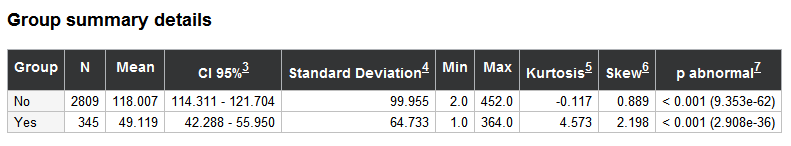
\includegraphics[width=\linewidth]{gfx/hyppara020}}
        \caption{Group Summary Details}
      \end{center}
    \end{figure}
    
    \begin{itemize}
      \item \textbf{Group}. For this exercise there were only two groups: ``No'' and ``Yes.''
      \item \textbf{N}. The number of observations in each group.
      \item \textbf{Mean}. The mean for each group.
      \item \textbf{CI $ 95\% $}. The $ 95\% $ confidence interval. For example, there is $ 95\% $ confidence that the actual mean for the ``No'' group lies between $ 114.311 $ and $ 121.704 $. 
      \item \textbf{Standard Deviation}. The standard deviation for each group.
      \item \textbf{Min}. The minimum value for each group.
      \item \textbf{Max}. The maximum value for each group.
      \item \textbf{Kurtosis}. The Kurtosis\footnote{Kurtosis and skew were described in Lab \ref{int:normal_distribution}, page \pageref{int:normal_distribution}.} for each group.
      \item \textbf{Skew}. This is a measure of the symmetry of the data. While it is problematic to categorically state that some value of skewness is ``bad,'' generally values lower than $ -1 $ or higher than $ +1 $ would be considered non-symmetrical. In the example calculated for this exercise, the ``No'' skew is $ +0.889 $ and would be considered reasonably symmetrical while the ``Yes'' skew is $ +2.198 $ and would be considered non-symmetrical.
      \item \textbf{p Abnormal}. This is a measure of the normality of the distribution. If the value is less than $ 0.05 $ then the data are not normally distributed. In the example calculated for this exercise, both groups have a value well below $ 0.05 $ and would be considered non-normally distributed. A histogram of each group's distribution is included in the ANOVA results and shown in the next two figures. It is easy to see that these data are not normally distributed.

      \begin{figure}[H]
        \begin{center}
          \fbox{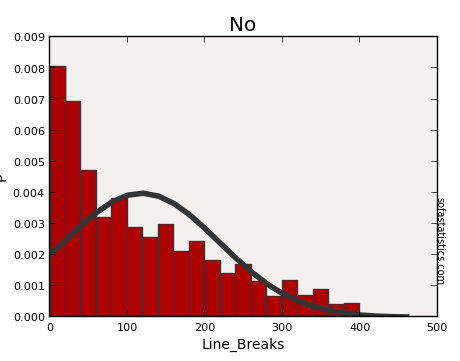
\includegraphics[width=\linewidth]{gfx/hyppara025}}
          \caption{``No'' Histogram}
          \label{hyp:no_histogram}
        \end{center}
      \end{figure}
    
      \begin{figure}[H]
        \begin{center}
          \fbox{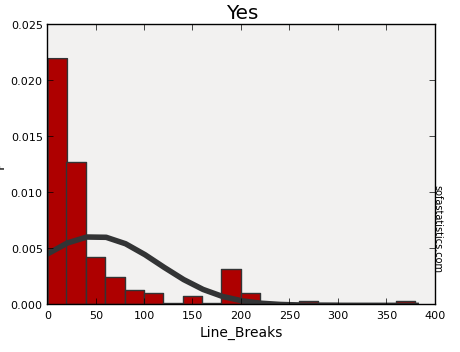
\includegraphics[width=\linewidth]{gfx/hyppara030}}
          \caption{``Yes'' Histogram}
        \end{center}
      \end{figure}
      
    \end{itemize}
    
  \end{enumerate}
  
  \item As another example where three groups are compared, consider an ANOVA using the ``email'' data, ``Line\_Breaks'' Averaged variable, and ``Attach'' as the ``Group By'' variable. For the grouped variable, choose to group from $ 0.0 $ to $ 2.0 $ only. Here are the results:
  
  \begin{figure}[H]
    \begin{center}
      \fbox{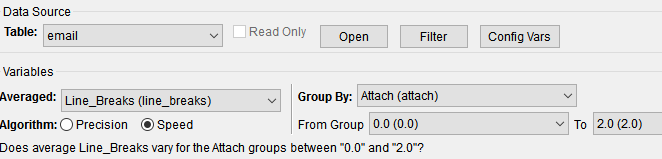
\includegraphics[width=\linewidth]{gfx/hyppara035}}
      \caption{Setting Up ANOVA for Attach}
    \end{center}
  \end{figure}

  \begin{figure}[H]
    \begin{center}
      \fbox{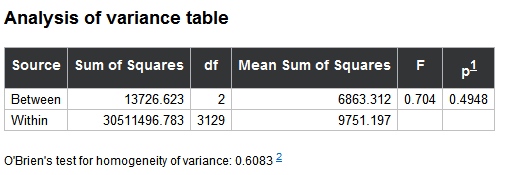
\includegraphics[width=\linewidth]{gfx/hyppara040}}
      \caption{ANOVA Table}
    \end{center}
  \end{figure}
  
  \begin{figure}[H]
    \begin{center}
      \fbox{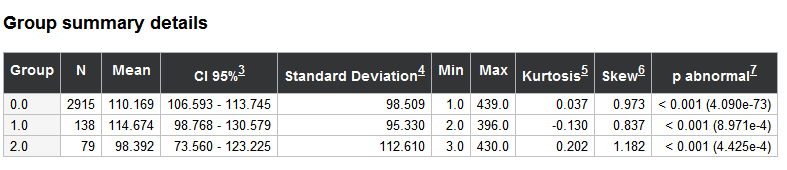
\includegraphics[width=\linewidth]{gfx/hyppara045}}
      \caption{ANOVA Group Summary}
    \end{center}
  \end{figure}
  
\end{enumerate}

\subsection{Activity 1: ANOVA} \label{para:act01}

Using the \textit{maincafe} dataset in \texttt{SOFA} conduct an ANOVA and report the Between Source \textit{p-value} for the following variables. Note: in the Word document submitted for this lab, Activity $ 1 $ should have a simple listing, something like this. (Notes: these are not the correct answers to the listed tests. To indicate tiny values use scientific notation in a form like $ 1.6e-5 $ since that is easier to type.)

\rowcolors{1}{}{}
\begin{center}
  \begin{tabular}{ll}
    $ 1 $ & $ 0.35 $ \\ 
    $ 2 $ & $ 1.27e-8 $ \\ 
    $ 3 $ & $ 237.4 $ \\ 
    $ 4 $ & $ 0.73 $ \\ 
  \end{tabular} 
\end{center}

Here are the variables to test:

\rowcolors{1}{gray!25}{}
\begin{center}
  \begin{tabular}{cllll}
    \hline 
    \textbf{Num} & \textbf{Averaged} & \textbf{Group By} & \textbf{From} & \textbf{To} \\ 
    \hline 
    $ 1 $ & Age & Food & $ 1.0 $ & $ 5.0 $ \\ 
    $ 2 $ & Age & Svc & $ 1.0 $ & $ 5.0 $ \\ 
    $ 3 $ & Age & Day & Friday & Wednesday \\ 
    $ 4 $ & Food & Day & Friday & Wednesday \\ 
    \hline 
  \end{tabular} 
\end{center}

\subsection{Correlation - Pearson's}

The Pearson's R statistic is covered in Lab \ref{cor:pearsons_r}, \nameref{cor:pearsons_r}, page \pageref{cor:pearsons_r}. The \texttt{SOFA} activity related to Pearson's R is on page \pageref{cor:pearsons_r_proc}.

\subsection{t-test - Independent}

\begin{enumerate}
  \item Start \texttt{SOFA} and click the "Statistics" button.
  \item Select "t-test - independent" from the Statistical Test list at the top of the window and then click the "Configure Test" button.
  \item Data Source Table: births
  \item Averaged Variable: Weight
  \item Group By Variable: Habit
  \item Group A: Nonsmoker
  \item Group B: Smoker
  
  \begin{figure}[H]
    \begin{center}
      \fbox{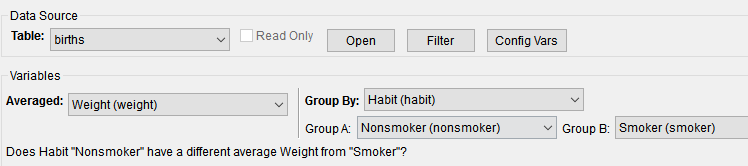
\includegraphics[width=\linewidth]{gfx/hyppara050}}
      \caption{Setting Up Independent t-Test}
    \end{center}
  \end{figure}
  
  \item Following is the result of that test.
  
  \begin{figure}[H]
    \begin{center}
      \fbox{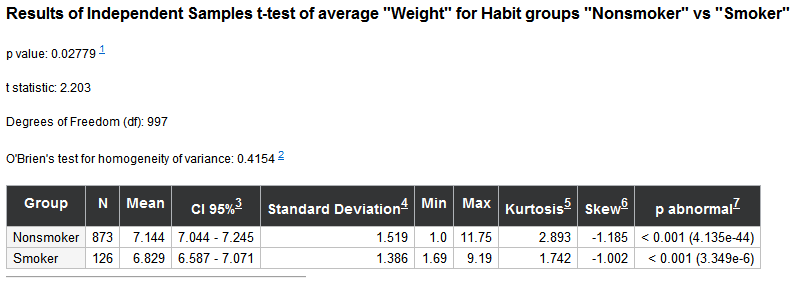
\includegraphics[width=\linewidth]{gfx/hyppara055}}
      \caption{Results of an Independent t-Test}
    \end{center}
  \end{figure}
  
  \item \textbf{p Value}. The most important statistic in the results window is the p-value. As always, when this number is encountered it is desired for it to have a value less than $ 0.05 $ ($ 5\% $). In the example calculated for this exercise, the p-value is $ 0.02779 $, which is less than $ 0.05 $, so there is a significant relationship between Birth Weight and Smoking Habit in this dataset.
  \item \textbf{t Statistic}. This number is of little value except, perhaps, to compare the results of one independent t-Test to another. In general, the greater the t-statistic the more likely the null hypothesis can be rejected, but it is challenging to find an appropriate ``cutoff'' score. Therefore, the most important result of an independent t-Test is the p-value.
  \item \textbf{Degrees of Freedom (df)}. The degrees of freedom is calculated as the number of different birth weights times one less than the number of groups.\footnote{The concept of Degrees of Freedom is explained in Lab \ref{cor:degrees_of_freedom}, page \pageref{cor:degrees_of_freedom}.}
  \item \textbf{O'Brien's Test}. This test is commonly used to indicate if the variances within two groups is significantly different. If the value of O'Brien's test is less than $ 0.05 $ ($ 5\% $) then the difference in the two variances is significant. In the example calculated for this exercise, O'Brien's test greater than $ 0.05 $ (at $ 0.4154 $), so the difference in the variance between the ``Nonsmoker'' and ``Smoker'' groups is not significant.
  \item \textbf{Other Statistics}. The table shows a number of statistical values for the two groups and each of the types of values have been described elsewhere.
  \item \textbf{Histograms}. The results window includes a histogram for each of the groups in the calculation, similar that that found for an ANOVA (see page \pageref{hyp:no_histogram}). Those histograms are not reproduced here.
  
\end{enumerate}

\subsection{Activity 2: t-test - Independent} \label{para:act02}

Using the \textit{maincafe} dataset in \texttt{SOFA} conduct a t-Test, Independent, and report the \textit{p-value} for the following variables. Note: in the Word document submitted for this lab, Activity $ 2 $ should have a simple listing, something like this. (Notes: these are not the correct answers to the listed tests. To indicate tiny values use scientific notation in a form like $ 1.6e-5 $ since that is easier to type.)

\rowcolors{1}{}{}
\begin{center}
  \begin{tabular}{ll}
    $ 1 $ & $ 0.35 $ \\ 
    $ 2 $ & $ 1.27e-8 $ \\ 
    $ 3 $ & $ 237.4 $ \\ 
    $ 4 $ & $ 0.73 $ \\ 
  \end{tabular} 
\end{center}

Here are the variables to test:

\rowcolors{1}{gray!25}{}
\begin{center}
  \begin{tabular}{cllll}
    \hline 
    \textbf{Num} & \textbf{Averaged} & \textbf{Group By} & \textbf{From} & \textbf{To} \\ 
    \hline 
    $ 1 $ & Age & Food & $ 1.0 $ & $ 5.0 $ \\ 
    $ 2 $ & Length & Meal & Breakfast & Other \\ 
    $ 3 $ & Miles & Sex & Female & Other \\ 
    $ 4 $ & Bill & Meal & Breakfast & Other \\ 
    \hline 
  \end{tabular} 
\end{center}

\subsection{t-test - Paired}

\begin{enumerate}
  \item Start \texttt{SOFA} and click the "Statistics" button.
  \item Select "t-test - paired" from the Statistical Test list at the top of the window and then click the "Configure Test" button.
  \item Data Source Table: tutoring
  \item Group A: Pretest
  \item Group B: Test\_1
  
  \begin{figure}[H]
    \begin{center}
      \fbox{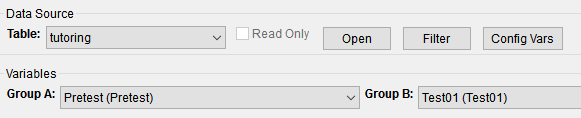
\includegraphics[width=\linewidth]{gfx/hyppara060}}
      \caption{Setting Up a Paired t-Test}
    \end{center}
  \end{figure}
  
  \item \texttt{SOFA} calculates the following result.
  
  \begin{figure}[H]
    \begin{center}
      \fbox{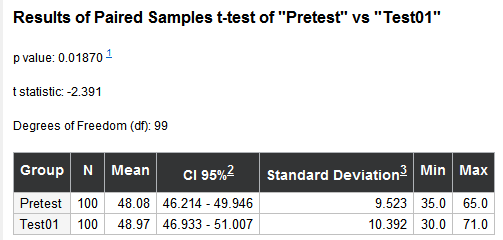
\includegraphics[width=\linewidth]{gfx/hyppara065}}
      \caption{Results of a Paired t-Test}
    \end{center}
  \end{figure}
  
  \item \textbf{p-Value}. As in all other statistical tests, the goal is a p-value less than $ 0.05 $ ($ 5\% $). In the example calculated for this exercise, the p-value is $ 0.01870 $, which is well below the $ 0.05 $ threshold, so the null hypothesis would be rejected.
  \item \textbf{t Statistic}. This number is of little value except, perhaps, to compare the results of one paired t-Test to another. In general, the greater the t-statistic the more likely the null hypothesis can be rejected, but it is challenging to find an appropriate ``cutoff'' score. Therefore, the most important result of an paired t-Test is the p-value.
  \item \textbf{Degrees of Freedom}. This is calculated as the number of observations minus one. Thus, $ 99 $ degrees of freedom indicate $ 100 $ observations in the dataset.
  \item \textbf{Other Statistics}. \texttt{SOFA} also calculates a number of statistics for each of the two groups, but those values are discussed elsewhere and will not be further covered here.
  \item \textbf{Graph}. \texttt{SOFA} also generates a graph of the results. In the following figure, the differences between pairs is graphed on the X-Axis. Ideally, the result would be a normal distribution, as indicated by the dark line. In this particular example, though, the results are rather flat which would indicate a possible problem with the experiment that the researcher would want to consider. 
  
  \begin{figure}[H]
    \begin{center}
      \fbox{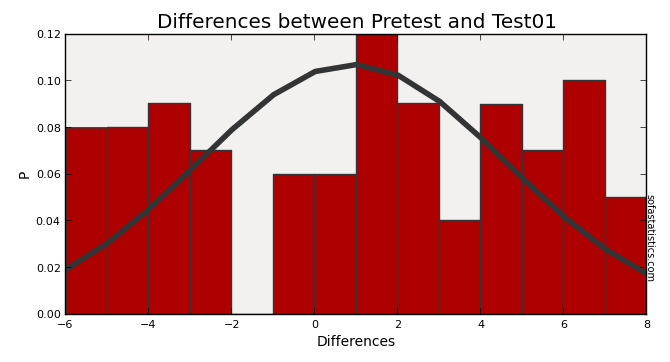
\includegraphics[width=\linewidth]{gfx/hyppara070}}
      \caption{Graphic Results of a Paired t-Test}
    \end{center}
  \end{figure}
  
\end{enumerate}

\section{Deliverable}

Complete the following activities in this lab:

\rowcolors{1}{gray!25}{}
\begin{center}
  \begin{tabular}{lll}
    \hline 
    \textbf{Number} & \textbf{Name} & \textbf{Page} \\ 
    \hline 
    \ref{para:act01} & \nameref{para:act01} & \pageref{para:act01} \\ 
    \ref{para:act02} & \nameref{para:act02} & \pageref{para:act02} \\ 
    \hline 
  \end{tabular} 
\end{center}

Consolidate the responses for all activities into a single document and submit that document for grading.


